\documentclass[a4paper,12pt]{article}

\usepackage[left=1.5cm,top=1.5cm,right=1.5cm,bottom=1.5cm,includehead,includefoot]{geometry}

\usepackage{cmap}
\usepackage[T2A]{fontenc}
\usepackage[utf8]{inputenc}
\usepackage[russian]{babel}
\usepackage[pdftex]{graphicx}
\usepackage{color}
\usepackage{ulem}
\usepackage{amsmath}
\usepackage{xcolor}
\usepackage{longtable}
\usepackage{hyperref}
\usepackage{import}
\usepackage{bytefield}
\usepackage{datetime}
\usepackage{float}
\usepackage{dirtree}
\usepackage{colortbl}
\usepackage{url}
\usepackage{multirow}
\graphicspath{{FIGURE/}}



\title{\Huge\textbf{Спецификация на ядро UART}}
\author{\huge RB}
\date{\today}

\pdfinfo{%
  /Title    (Спецификация на ядро UART)
  /Author   (RB)
  /Creator  (RB)
  /Producer (RB)
  /Subject  (IP-core specification)
  /Keywords (SystemVerilog, FPGA, UART, IP-core)
}


\begin{document}
\maketitle
\newpage


%
% --Список фигур---
%
\listoffigures
\addcontentsline{toc}{chapter}{\listfigurename}
\newpage

% --Список таблиц---
%
\listoftables
\addcontentsline{toc}{chapter}{\listtablename}
\newpage


%
%---Chapters----
%
%
% Introduction
%
\section{Введение}
\label{sec:introduction}

Данная спецификация описывает ядро UART, управление которым осуществляется при помощи интерфейса Avalon-MM или, в перспективе, AXI Lite (на данный момент находится в стадии разработки).

    \subsection{Интеграция}
    Изначально ядро предполагает интеграцию в QSYS САПР Quartus, но никто не запрещает добавлять его в любой другой дизайн. Пример интеграции показан на рисунке \ref{img:integrated_ip}

    \begin{figure}[H]
        \centering
        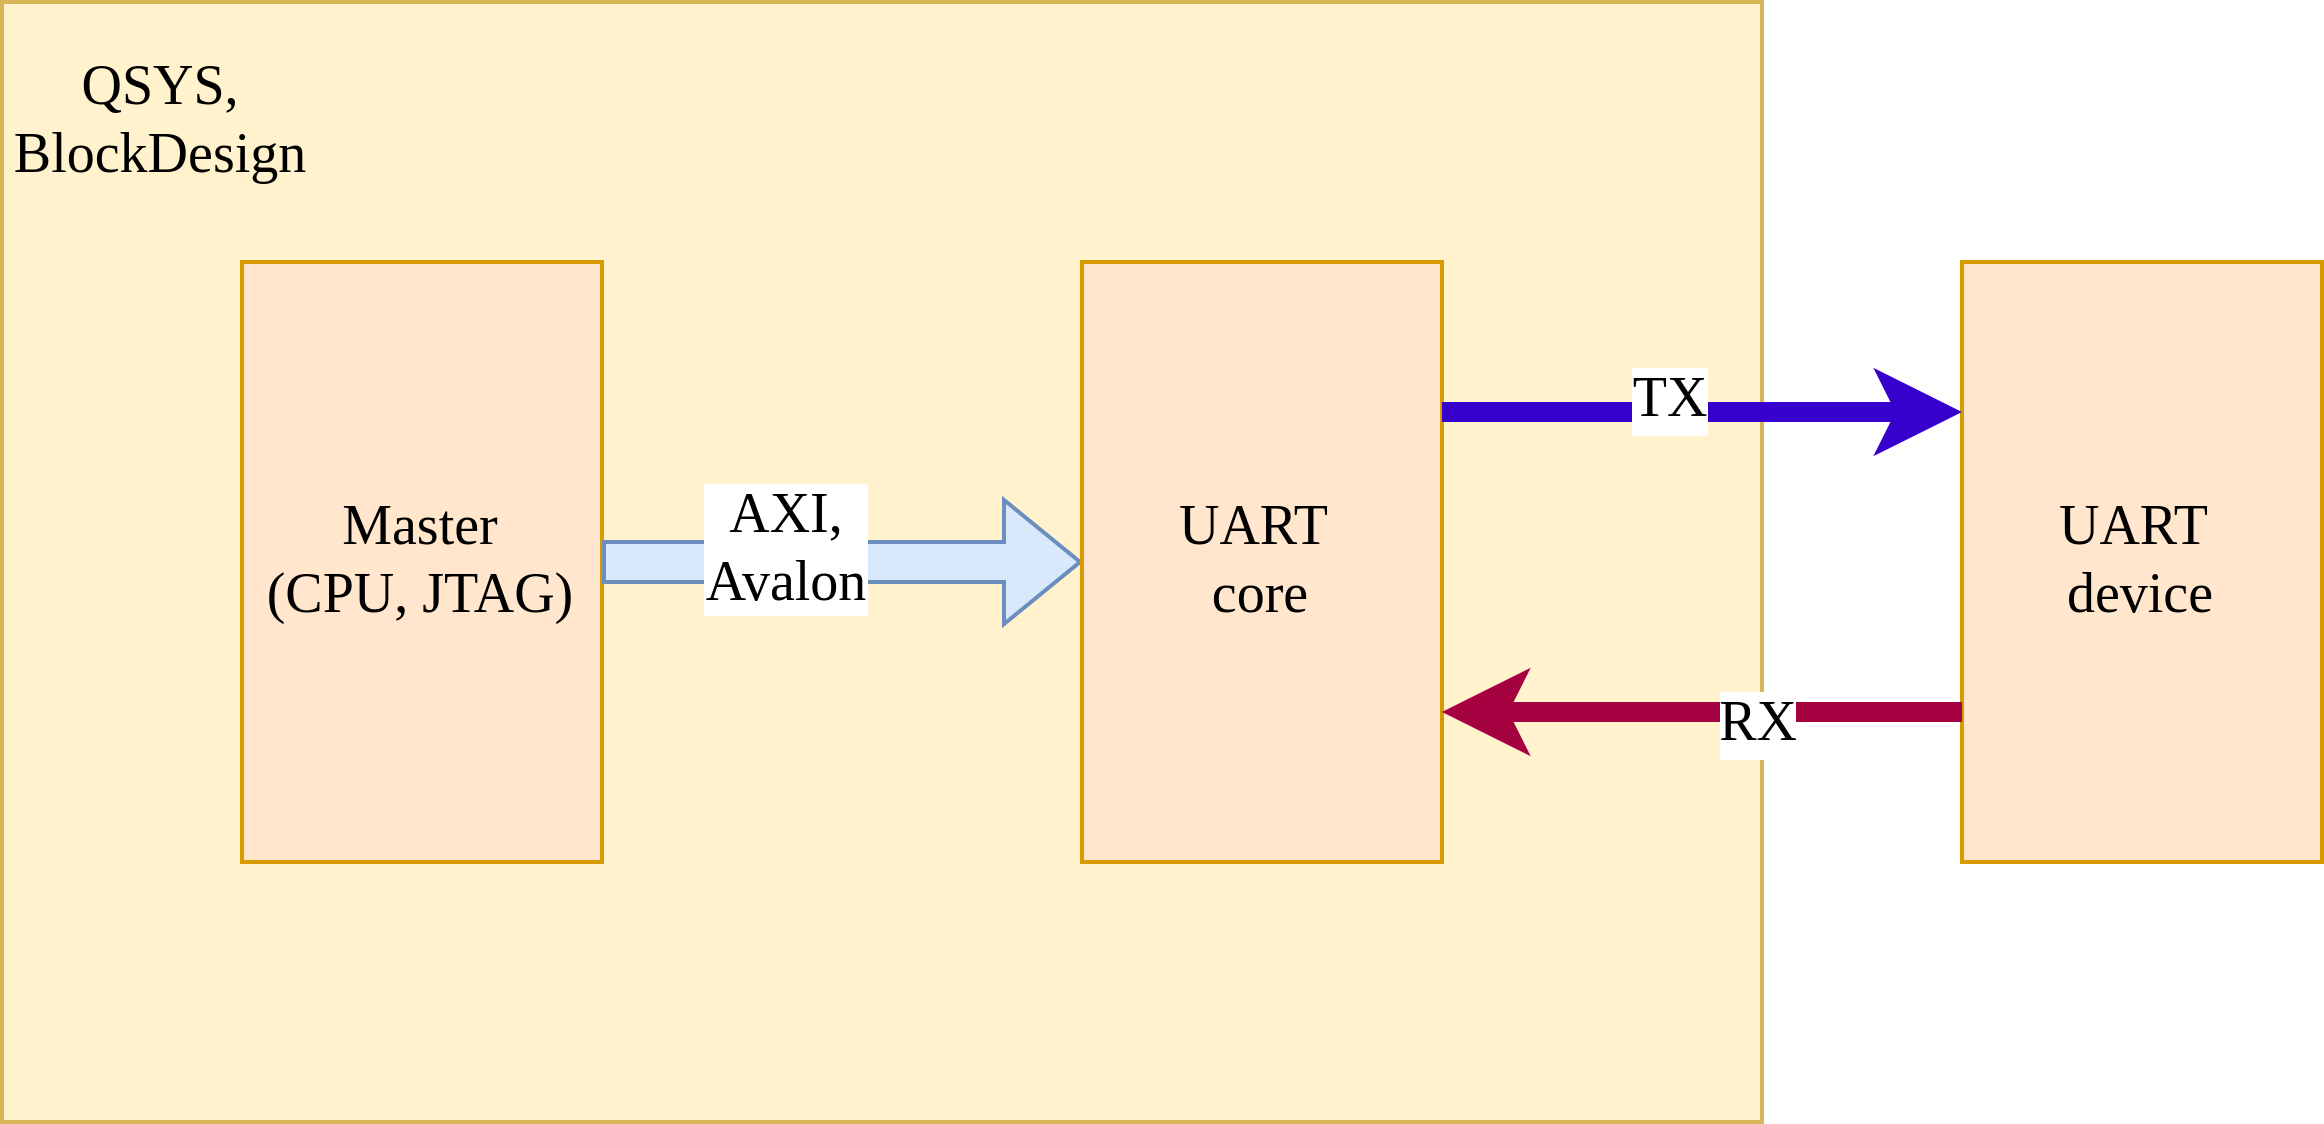
\includegraphics[width=15cm]{Integrate.png}
        \caption{Пример интеграции ядра в SoC}
        \label{img:integrated_ip}
    \end{figure}


    \subsection{Описание сигналов}

    В таблице \ref{tab:descr_singals} перечислены сигналы модуля для связи с внешним миром.

    \begin{table}
        \caption{Описание сигналов}
        \begin{center}
            \begin{tabular}{l|l|l|l}
                    \rowcolor[gray]{0.7} Имя & Направление & Ширина & Описание \\ \hline \hline
                    \multicolumn{4}{c}{Глобальные сигналы} \\ \hline
                    \texttt{clk} & input & 1 & тактовый сигнал для работы модуля \\ \hline
                    \texttt{reset\_n} & input & 1 & асинхронный сброс по заднему фронту \\ \hline

                    \multicolumn{4}{c}{Интерфейс Avalon-MM Slave} \\ \hline
                    \texttt{avmms\_write\_i} & input & 1 & write \\ \hline
                    \texttt{avmms\_address\_i} & input & 3 & address \\ \hline
                    \texttt{avmms\_writedata\_i} & input & 32 & writedata \\ \hline
                    \texttt{avmms\_byteenable\_i} & input & 4 & byteenable \\ \hline
                    \texttt{avmms\_read\_i} & input & 1 & read \\ \hline
                    \texttt{avmms\_waitrequest\_o} & output & 1 & waitrequest \\ \hline
                    \texttt{avmms\_readdata\_o} & output & 32 & readdata \\ \hline

                    \multicolumn{4}{c}{Интерфейс UART} \\ \hline
                    \texttt{uart\_rx} & input & 1 & линия RX \\ \hline
                    \texttt{uart\_tx} & output & 1 & линия TX \\ \hline
                    \hline
            \end{tabular}
            \label{tab:descr_singals}
        \end{center}
    \end{table}



    \subsection{Возможности ядра}
    Данное ядро обладает следующими возможностями:
    \begin{itemize}
     \item поддержка интерфейсов Avalon-MM и AXI Lite;
     \item программная установка любого BaudRate, в том числе не из таблицы стандартных скоростей;
     \item программное включение бита четности;
     \item поддержка odd и even битов четности;
     \item возможность установки до четырех стоп-битов
     \item настраиваемый размер приемного и передающего буферов.
    \end{itemize}


\newpage
\section{Использование}
\subsubsection{Структура директорий}
  Проект содержит имеет следующую структуру директории:

    \dirtree{%
        .1 ..
        .2 RTL.
        .2 SIM.
        .2 OTHER.
        .2 DOC.
        .3 FIGURE.
    }

\begin{description}
    \item[\texttt{RTL}] - исходники ядра на языках Verilog и SystemVerilog,
    \item[\texttt{SIM}] - файлы для симуляции. \textbf{uart\_mm\_top\_tb.sv} - тестбенч для симуляции всего ядра. Для него предназначен \textbf{uart\_mm\_top\_wave.do} - скрипт для инициализации окна \textbf{wave} в \textbf{ModelSim/QuestaSim}). \textbf{uart\_tb.sv} - тестбенч для симуляции только приемопередатчика (проверка битов четности, стоп-битов и т.д.). Для него предназначен \textbf{wave.do} - скрипт для инициализации окна \textbf{wave} в \textbf{ModelSim/QuestaSim})
    \item[\texttt{OTHER}] - для прочих файлов, содержит таблицу стандартных скоростей,
    \item[\texttt{DOC}] - документация на ядро. Исходники в формате \TeX,
    \item[\texttt{DOC/FIGURE}] - хранилище изображений.
\end{description}

\newpage
\section{Архитектура}

На рисунке \ref{img:design_ip} представлена архитектура IP-ядра и основные пути следования данных.

    \begin{figure}[H]
        \centering
        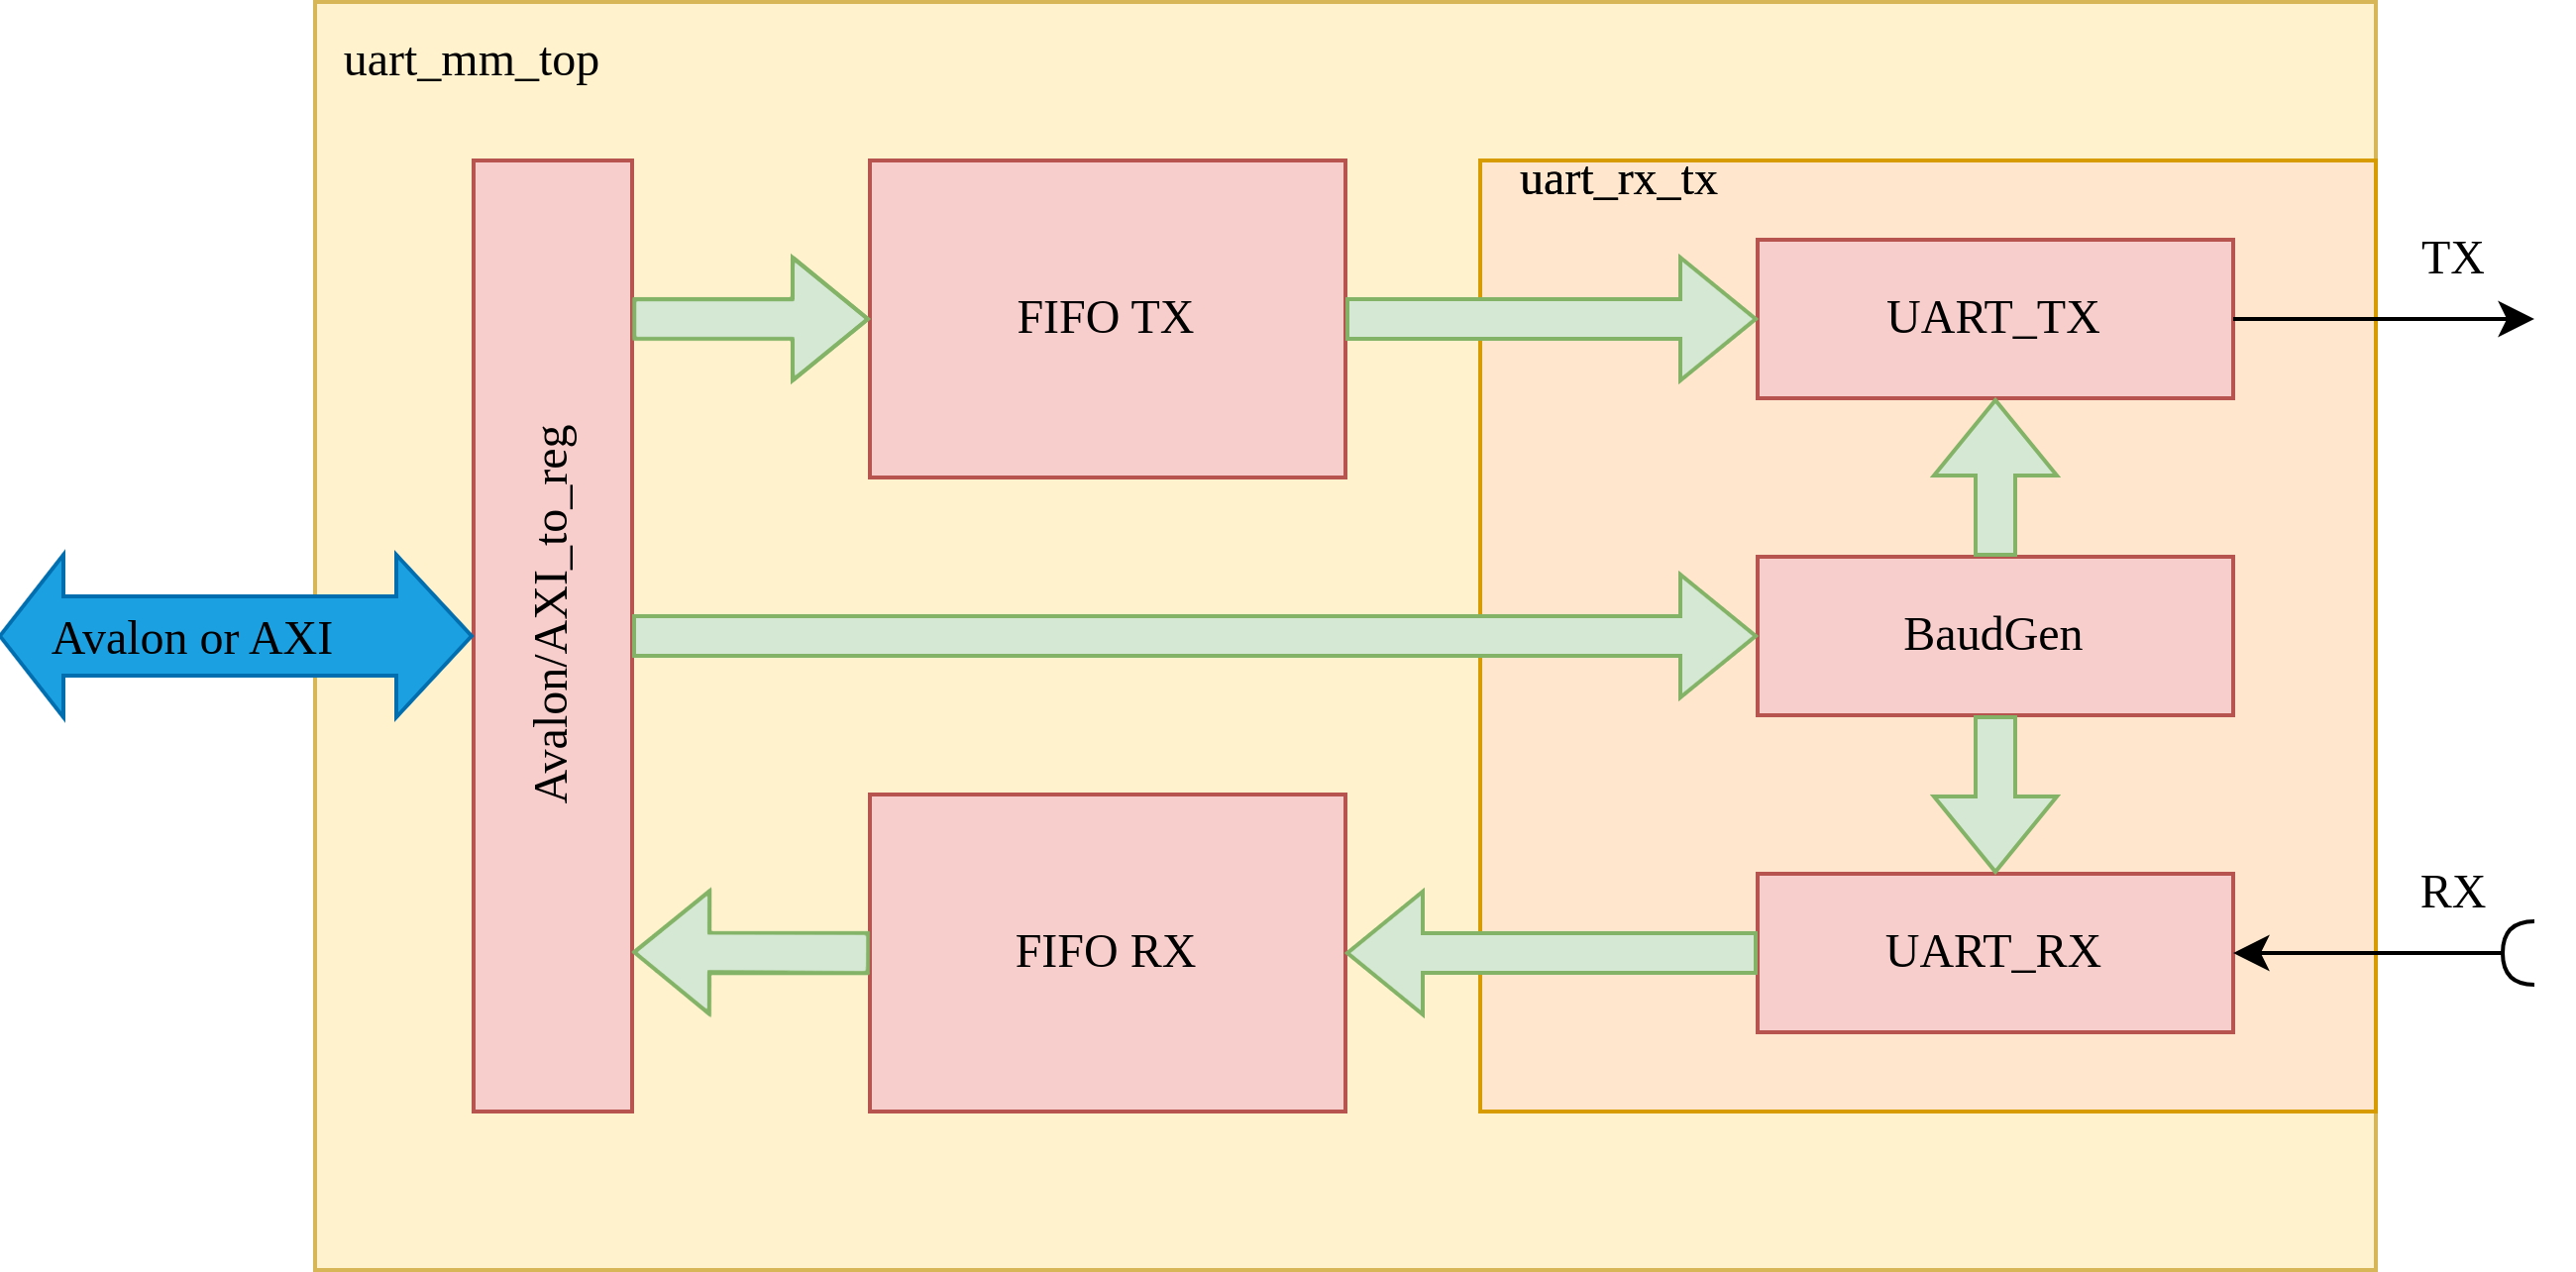
\includegraphics[width=15cm]{DesignIP.png}
        \caption{Архитектура IP-ядра}
        \label{img:design_ip}
    \end{figure}

Рассмотрим процесс передачи. Через интерфейс \textbf{Avalon} или \textbf{AXI} пользователь осуществляет запись байта в регистр \textbf{TX\_FIFO}(см. п. \ref{sec:register_map}), далее байт для записи попадает в очередь на передачу - \textbf{FIFO\_TX}. Данные из \textbf{FIFO\_TX} попадают на модуль \textbf{UART\_TX}, где происходит их сериализация и выдача на линию \textbf{TX}. Модуль \textbf{BaudGen} осуществляет генерацию сигналов для выдачи данных (и приема) на частоте, которую задает пользователь (например 9600 бод).
Процесс приема аналогичен процессу передачи. Модуль \textbf{UART\_RX} фиксирует стартовый бит посылки и начинает десериализацию данных в зависимости от параметров, выставленных пользователем (наличие бита четности и количество стоповых бит). Десериализованный байт попадает в \textbf{FIFO\_RX}, заодно выполняется проверка бита четности (если последний включен в регистре \textbf{CONTROL}) и результат так же записывается в \textbf{FIFO\_RX}.




\newpage
\section{Карта регистров}
\label{sec:register_map}

Модуль имеет 6 регистров управления, представленные в таблице {\ref{tbl:uart_regs}}. В таблице приняты следующие обозначения: RO - Read Only (только для чтения), WO - Write Only (только для записи), WR - Write or Read (чтение и запись). Default - значение, принимаемое регистром после сброса.

\begin{table}[H]
  \begin{center}
    \begin{tabular}{l|c|c|c|l}
      \rowcolor[gray]{0.7} {\tt Имя} & {\tt Адрес, DW} & {\tt Ширина} & {\tt Доступ} & {\tt Описание} \\ \hline \hline
      {\tt CONTROL}   & 3'b000 & 32 & RW & Управление параметрами передачи\\ \hline
      {\tt BAUD}      & 3'b001 & 32 & RW & Установка BaudRate\\ \hline
      {\tt FILL\_TX}  & 3'b010 & 32 & RO & Число байт, ожидающих передачи из TX FIFO\\ \hline
      {\tt FILL\_RX}  & 3'b011 & 32 & RO & Число байт, ожидающих чтения из RX FIFO\\ \hline
      {\tt TX\_FIFO}   & 3'b100 & 32 & WO & Запись байт в буфер передачи\\ \hline
      {\tt RX\_FIFO}   & 3'b101 & 32 & RO & Чтение байт из буфера приема\\ \hline
    \end{tabular}
    \caption{Регистры управления ядра UART}
    \label{tbl:uart_regs}
    \end{center}
\end{table}

\subsection{CONTROL}

Регистр \textbf{CONTROL} служит для управления процессами приема, передачи и контроля за флагами приемного и передающего FIFO.

\begin{table}[H]
  \begin{center}
    \begin{tabular}{l|c|c|l}
      \rowcolor[gray]{0.7}{\tt Bit} & {\tt Access} & {\tt Default} & {\tt Decription} \\\hline\hline
      {\tt [0]} & RO & 1'b1 & FIFO TX Empty \\ \hline
      {\tt [1]} & RO & 1'b0 & FIFO TX Full \\ \hline
      {\tt [2]} & RO & 1'b1 & FIFO RX Empty \\ \hline
      {\tt [3]} & RO & 1'b0 & FIFO RX Empty \\ \hline
      {\tt [7:4]} & RO & 4'b0 & Reserved \\ \hline

      {\tt [8]} & RW & 1'b0 & Enable parity bit \\ \hline
      {\tt [9]} & RW & 1'b0 & Type parity bit\\ \hline
      {\tt [11:10]} & RW & 2'b0 & Count stop bits \\ \hline

      {\tt [12]} & RW & 1'b1 & Enable transmitter \\ \hline
      {\tt [13]} & RW & 1'b1 & Enable receiver \\ \hline
    \end{tabular}
    \caption{Биты регистра CONTROL}
    \label{tbl:control_bits}
    \end{center}
\end{table}


\textbf{FIFO TX Empty} - данный бит выставляется в единицу если FIFO TX не содержит никаких данных для передачи.

\textbf{FIFO TX Full} - данный бит выставляется в единицу если FIFO TX заполнено. Данные, записываемые в FIFO TX при установленном флаге, будут потеряны.

\textbf{FIFO RX Empty} - данный бит выставляется в единицу если FIFO RX не содержит данных для чтения.

\textbf{FIFO RX Full} - данный бит выставляется в единицу если FIFO RX заполнено. Все данные, которые в дальнейшем будут приняты от UART не запишутся и будут утеряны.

\textbf{Enable parity bit} - включение бита четности.

\textbf{Type parity bit} - тип бита четности, 1'b0 - EVEN, 1'b1 - ODD.

\textbf{Count stop bits} - количество стоповых бит: 2'b00 - 1, 2'b01 - 2, 2'b10 - 3, 2'b11 - 4;

\textbf{Enable transmitter} - данный бит разрешает работу ядра на передачу по UART. В случае отключения передатчика поступающие данные будут накапливаться в FIFO TX.

\textbf{Enable receiver} - данный бит разрешает работу ядра на прием по UART. В случае отключения приемника, принимемые данные по UART не будут записываться в FIFO RX, а будут отбрасываться.


\subsection{BAUD}

Данный 32-битный регистр служит для управления скоростью, на которой работает приемник и передатчик UART. Значение регистра вычисляется согласно следующему выражению: $$BAUD = round\left(\frac{SystemClock}{8*BaudRate}\right)-1,$$ где $SystemClock$ - тактовая частота работы модуля в Гц, $BaudRate$ - скорость UART в бодах (например, стандартная табличная), $round()$ - операция округления.

\subsection{FILL\_TX}

Данный 32-битный регистр указывает количество байт, которые находятся в FIFO TX и ожидают передачи по UART.  При попадании байта в FIFO\_TX происходит увеличение счетчика FILL\_TX на единицу. Если модуль UART\_TX забирает байт из FIFO\_TX для передачи, то FILL\_TX уменьшается на единицу и т.д.

\subsection{FILL\_RX}

Данный 32-битный регистр указывает количество байт, принятых по UART и ожидающих чтения из FIFO RX. При попаданиие байта из модуля UART\_RX в FIFO RX происходит увеличение счетчика FILL\_RX на единицу. Если пользователь читает байт из FIFO RX путем доступа к регистру RX\_FIFO, то счетчик FILL\_RX уменьшается на единицу и т.д.

\subsection{TX\_FIFO}

Данный регистр служит для записи передаваемых байт в FIFO TX. Для того, чтобы поместить байт $byte[7:0]$ в FIFO TX для последующей передачи, необходимо записать его в данный регистр. Ядро принимает для передачи только младшие 8 бит - $TX\_FIFO[7:0]$, игнорируя остальные. Так что не важно, мастер какой ширины управляет модулем (32-,16-,8-битный).

\subsection{RX\_FIFO}

Данный регистр служит для чтения байт из FIFO RX. Поддерживается только одновременное чтение одного байта из FIFO RX (burst не поддерживается). При чтении $RX\_FIFO[7:0]$ возвращает прочитанный из FIFO RX байт, $RX\_FIFO[8]$ возвращает статус проверки бита четности - $1'b1$ в случае ошибки. Данный бит всегда принимает нулевое значение в случае если бит четности отключен в регистре \textbf{CONTROL}.


\end{document}
